% ============ Import Library ============
% Apply template
\documentclass[a4paper,oneside]{article}
% Using vietnamese
\usepackage[utf8]{vietnam}
\usepackage[vietnamese=nohyphenation]{hyphsubst}
\usepackage[vietnamese]{babel}
\usepackage[utf8]{inputenc}
% Some essential libs for math
\usepackage{amsmath, amsfonts, amssymb}
\usepackage{mathtools}
\usepackage{cases}
\usepackage{commath}
\usepackage{mathrsfs}
\usepackage{enumerate}
% Essential libs for paper format
\usepackage{graphicx}
\usepackage{scrextend}
\usepackage[margin=1.0in]{geometry}
\usepackage[explicit]{titlesec}
% Others
\usepackage{fancyhdr}
\usepackage{lipsum}
\usepackage{tikz, tcolorbox}
% Font style
\usepackage{mathptmx}
\usepackage[T1]{fontenc}

% ============ Configs ============
% paper formats
\changefontsizes{12pt}
\setlength{\topmargin}{-0.8in}
\setlength{\textheight}{9.25in}
\renewcommand{\baselinestretch}{1.2}
\titlespacing{\section}{0pt}{12pt}{2pt}
\DeclareTextFontCommand{\textbfit}{\bfseries\itshape}
\setlength{\parindent}{0pt}
% Define commands
\renewcommand{\leq}{\leqslant}
\renewcommand{\geq}{\geqslant}
\newcommand{\nl}{\\[1.5mm]}
\newcommand{\nll}{\\[2.0mm]}
\newcommand{\nlll}{\\[3.0mm]}
\newcommand{\dlim}{\displaystyle\lim}
\newcommand{\N}{\mathbb N}
\newcommand{\Z}{\mathbb Z}
\newcommand{\Q}{\mathbb Q}
\newcommand{\R}{\mathbb R}
\newcommand{\C}{\mathbb C}
\DeclareMathOperator{\Ima}{Im}
\newcommand*{\QED}[1][$\square$]{%
\leavevmode\unskip\penalty9999 \hbox{}\nobreak\hfill
    \quad\hbox{#1}%
}
\newcommand*{\QEDFill}{\null\nobreak\hfill\ensuremath{\blacksquare}}
\newcommand{\startproof}{\begin{center}Giải\end{center}}

\makeatletter
\newenvironment{sqcases}{%
  \matrix@check\sqcases\env@sqcases
}{%
  \endarray\right.%
}
\def\env@sqcases{%
  \let\@ifnextchar\new@ifnextchar
  \left\lbrack
  \def\arraystretch{1.2}%
  \array{@{}l@{\quad}l@{}}%
}
\makeatother
% Exercise env
\newenvironment{exercise}[1]{
	\begin{tcolorbox}
	\textbf{Bài #1:}}{
	\end{tcolorbox}
}
\newenvironment{proof}{\startproof
}{\QEDFill\\}

% ============ Meta data ============
\title{\textbf{Bài tập giải tích 2 - Chương 1}}
\author{Nguyễn Đình Đăng Khoa (MSSV: 20110217)}
\date{Ngày 2 Tháng 11 Năm 2021}


\begin{document}

% Cover

\newgeometry{margin=0.5in, top=0.5in}
%% temporary titles
% command to provide stretchy vertical space in proportion
\newcommand\nbvspace[1][3]{\vspace*{\stretch{#1}}}
% allow some slack to avoid under/overfull boxes
\newcommand\nbstretchyspace{\spaceskip0.5em plus 0.25em minus 0.25em}
% To improve spacing on titlepages
\newcommand{\nbtitlestretch}{\spaceskip0.6em}
\thispagestyle{empty}
\begin{tcolorbox}
\begin{center}

\vspace{1.2cm}
\centerline{ĐẠI HỌC QUỐC GIA TP.HCM}
\centerline{\bf\underline{TRƯỜNG ĐẠI HỌC KHOA HỌC TỰ NHIÊN}}
\vspace{2.8cm}

\nbvspace[1]
\Huge
{\huge\textbf{
BÀI TẬP GIẢI TÍCH 2 - CHƯƠNG I}}

\normalsize

\vspace{0.5cm}

\small BY\\[0.6em]
\Large NGUYỄN ĐÌNH ĐĂNG KHOA\\
\Large (MSSV: 20110217)

\vspace{2.8cm}

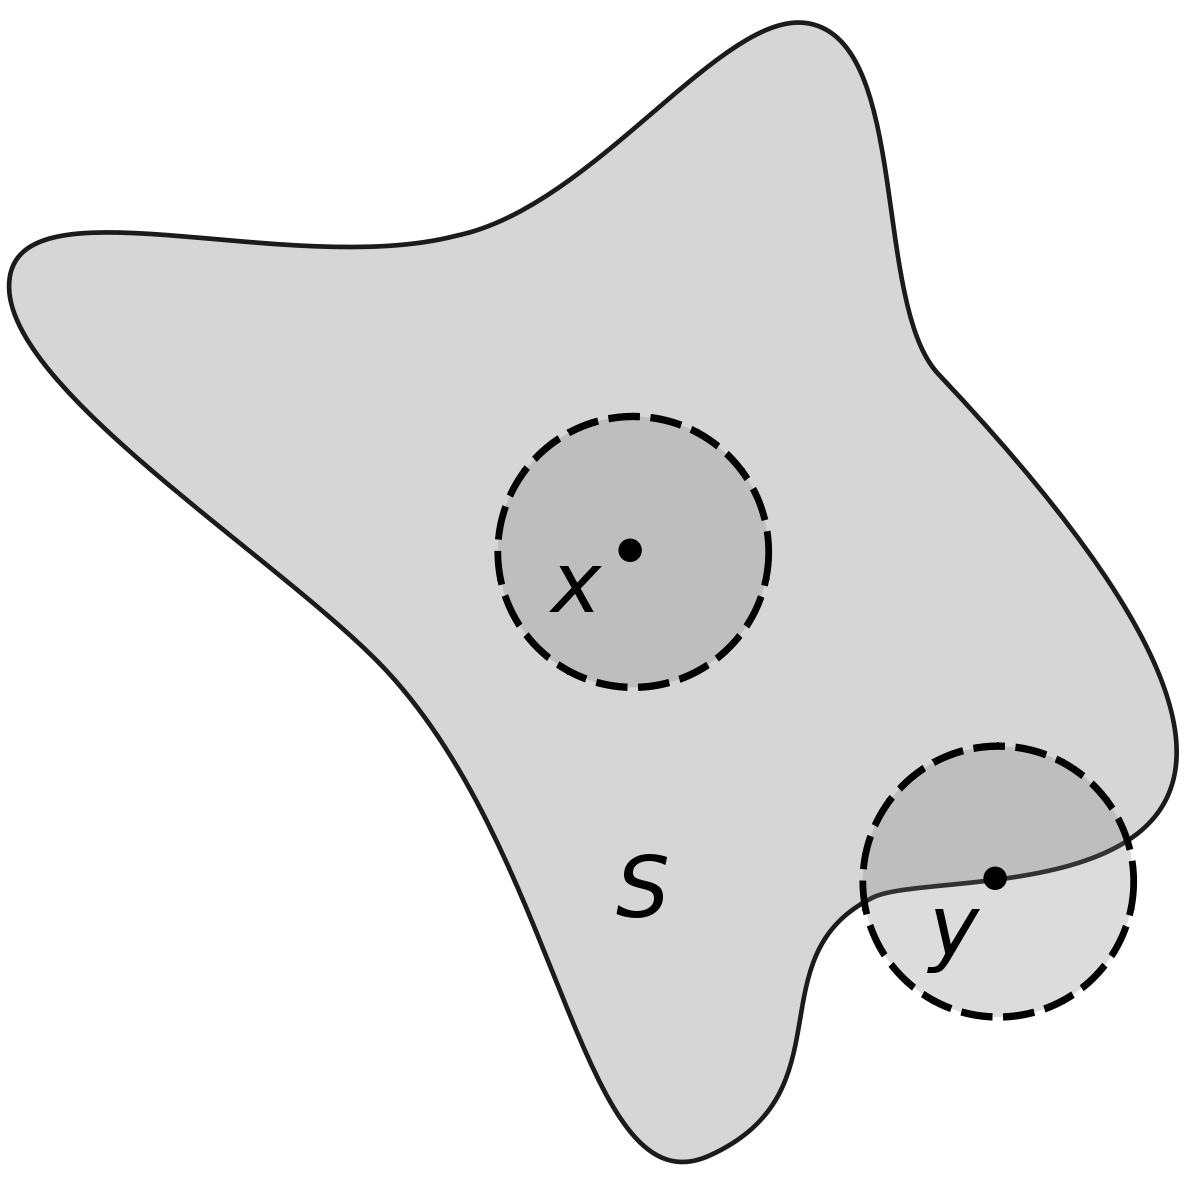
\includegraphics[width=3.5in]{./assets/interior-bw}

\vspace{2.9cm}

\normalsize

% \textbf{
TP. Hồ Chí Minh - Ngày 2 tháng 11 năm 2021
% }
\vspace{1.5cm}
\nbvspace[1]

\end{center}
\end{tcolorbox}

\pagebreak
\clearpage
\restoregeometry
% }

\begin{exercise}{1}
	Cho $(X,\|.\|)$ là một không gian định chuẩn. Chứng minh rằng ánh xạ $d: X \times X \rightarrow \R$, xác định bởi $d(x,y)=\|x-y\|$ là một metric trên $X$.
\end{exercise}

\begin{proof}
Ta có với mọi $x, y, z \in X$ thì
\begin{itemize}
    \item $d(x,y)=\|x-y\| \geq 0$ và $d(x,y)=\|x-y\|=0 \Leftrightarrow x-y = 0 \Leftrightarrow x = y$
    \item $d(x,y)=\|x-y\|=\abs{-1}\cdot\|y-x\|=d(y,x)$
    \item $\|.\|$ thoả các bất đẳng thức tam giác sau \nl
    $\begin{cases}
        \|x-z\| \leq \|x\| + \|z\|\\
        \|x-y\| \leq \|x\| + \|y\|\\
        \|y-z\| \leq \|y\| + \|z\|\\
    \end{cases}$\nl
    $\Rightarrow \|x-z\| - \|x-y\| - \|y-z\| \leq -2\|y\| \leq 0$\\
    $\Rightarrow \|x-z\| \leq \|x-y\| + \|y-z\|$
\end{itemize}
Vậy $(X,d)$ là một không gian metric.
\end{proof}

\begin{exercise}{2}
	\\$a)$ Cho $(X,d)$ là một không gian metric. Chứng minh
	$$
	\abs{d(x,a)-d(y,a)} \leq d(x,y),\ \text{với mọi } x, y, a \in X.
	$$
	$b)$ Cho $(X,\|.\|)$ là một không gian định chuẩn. Chứng minh
	$$
	\abs{ \|x\| - \|y\| } \leq \|x-y\|,\ \text{với mọi } x, y \in X.
	$$
\end{exercise}

\begin{proof}
$a)$ Với mọi $x, y, a \in X$ thì
$$
    \abs{d(x,a)-d(y,a)} \leq \abs{d(x,a)+d(a,y)} \leq \abs{d(x,y)} = d(x,y).
$$
$b)$ Với mọi $x, y \in X$ thì ta có
\begin{alignat*}{3}
    & & \|x\| = \|x-y+y\| &\leq \|x-y\| + \|y\|\\
    & \Rightarrow &\|x\| - \|y\| &\leq \|x-y\|. \tag{1}
\end{alignat*}
và
\begin{alignat*}{3}
    & & \|y\| = \|y-x+x\| &\leq \|y-x\| + \|x\|\\
    & \Rightarrow &\ \ -\|y - x\| = -\|x - y\| &\leq \|x\| - \|y\|. \tag{2}
\end{alignat*}
Từ $(1)$ và $(2)$ suy ra $\abs{ \|x\| - \|y\| } \leq \|x-y\|,\ \text{với mọi } x, y \in X$.
\end{proof}

\begin{exercise}{3}
    Chứng minh rằng các hàm số
    \begin{align*}
        &\|\mathbf{x}\|_2 = \sqrt{x_1^2+\cdots+x_n^2},\\
        &\|\mathbf{x}\|_1 = \abs{x_1}+\cdots+|x_n|,\\
        &\|\mathbf{x}\|_{\infty} = \max_{i = 1,\cdots,n} |x_i|,
    \end{align*}
    với $\mathbf{x} = (x_1,\cdots,x_n) \in \R^n$, là các chuẩn trên $\R^n$.
\end{exercise}

\begin{proof}
Xét $\|\mathbf{.}\|_2$, ta có với mọi $\mathbf{x}, \mathbf{y} \in \R^n, \alpha \in \R$ thì
\begin{itemize}
    \item $\|\mathbf{x}\|_2 = \sqrt{x_1^2+\cdots+x_n^2} \geq 0$
        và $\sqrt{x_1^2+\cdots+x_n^2} = 0 \Leftrightarrow x_1 = x_2 = \cdots = x_n = 0 \Leftrightarrow \mathbf{x} = 0$.
    \item $\|\mathbf{\alpha x}\|_2 = \sqrt{(\alpha x_1)^2+\cdots+(\alpha x_n)^2} = \abs{\alpha} \sqrt{x_1^2+\cdots+x_n^2} = \abs{\alpha} \|\mathbf{x}\|_2$.
    \item Xét biến đổi tương đương sau
    \begin{alignat*}{3}
        & & \|\mathbf{x} + \mathbf{y}\|_2 &\leq \|\mathbf{x}\|_2 + \|\mathbf{y}\|_2\\
        &\Leftrightarrow\ & \sqrt{(x_1+y_1)^2+\cdots+(x_n+y_n)^2} &\leq \sqrt{x_1^2+\cdots+x_n^2} + \sqrt{y_1^2+\cdots+y_n^2}\\
        &\Leftrightarrow\ & (x_1+y_1)^2+\cdots+(x_n+y_n)^2 &\leq x_1^2+\cdots+x_n^2 + y_1^2+\cdots+y_n^2 + 2\sqrt{x_1^2+\cdots+x_n^2} \cdot \sqrt{y_1^2+\cdots+y_n^2}\\
        &\Leftrightarrow\ & 2(x_1y_1+\cdots+x_ny_n) &\leq 2\sqrt{x_1^2+\cdots+x_n^2} \cdot \sqrt{y_1^2+\cdots+y_n^2}\\
        &\Leftrightarrow\ & (x_1y_1+\cdots+x_ny_n)^2 &\leq (x_1^2+\cdots+x_n^2) \cdot (y_1^2+\cdots+y_n^2)
    \end{alignat*}\\[-0.8cm]
    % \begin{center}
        (Luôn đúng do bất đẳng thức Bunhiacopxki)
    % \end{center}
\end{itemize}
Vậy từ các tính chất trên ta suy ra $\|\mathbf{.}\|_2$ là một chuẩn trên $\R^n$.\QEDFill\nll
Xét $\|\mathbf{.}\|_1$, ta có với mọi $\mathbf{x}, \mathbf{y} \in \R^n, \alpha \in \R$ thì
\begin{itemize}
    \item $\|\mathbf{x}\|_1 = |x_1|+\cdots+|x_n| \geq 0$
        và $|x_1|+\cdots+|x_n| = 0 \Leftrightarrow x_1 = x_2 = \cdots = x_n = 0 \Leftrightarrow \mathbf{x} = 0$.
    \item $\|\mathbf{\alpha x}\|_1 = |\alpha x_1|+\cdots+|\alpha x_n| = \abs{\alpha} (|x_1|+\cdots+|x_n|) = \abs{\alpha} \|\mathbf{x}\|_1$.
    \item $\|\mathbf{x}+\mathbf{y}\|_1 = \abs{x_1 + y_1} + \cdots + \abs{x_n + y_n} \leq (\abs{x_1} + \cdots + \abs{x_n}) + (\abs{y_1} + \cdots + \abs{y_n}) = \|\mathbf{x}\|_1+\|\mathbf{y}\|_1$.
\end{itemize}
Vậy từ các tính chất trên ta suy ra $\|\mathbf{.}\|_1$ là một chuẩn trên $\R^n$.\QEDFill\nll
Xét $\|\mathbf{.}\|_{\infty}$, ta có với mọi $\mathbf{x}, \mathbf{y} \in \R^n, \alpha \in \R$ thì
\begin{itemize}
    \item $\|\mathbf{x}\|_{\infty} = \displaystyle\max_{i = 1,\cdots,n} |x_i| \geq 0$
        và vì $\abs{x_i}$ luôn lớn hơn $0$ và có giá trị nhỏ nhất bằng $0$ nên\\$\displaystyle\max_{i = 1,\cdots,n} |x_i| = 0 \Leftrightarrow x_1 = x_2 = \cdots = x_n = 0 \Leftrightarrow \mathbf{x} = 0$.
    \item $\|\mathbf{\alpha x}\|_{\infty} = \displaystyle\max_{i = 1,\cdots,n} |\alpha x_i| = \abs{\alpha}\displaystyle\max_{i = 1,\cdots,n} |x_i| = \abs{\alpha} \|\mathbf{x}\|_{\infty}$.
    \item Ta có $\abs{x_i + y_i} \leq \abs{x_i} + \abs{y_i}$ với mọi $i = 1\cdots n$ nên
    \begin{alignat*}{3}
        & & \max_{i = 1,\cdots,n} |x_i + y_i| &\leq \max_{i = 1,\cdots,n} (|x_i| + |y_i|) \leq \max_{i = 1,\cdots,n} |x_i| + \max_{i = 1,\cdots,n} |y_i| \\
        &\Leftrightarrow\ & \|\mathbf{x} + \mathbf{y}\|_{\infty} &\leq \|\mathbf{x}\|_{\infty} + \|\mathbf{y}\|_{\infty}.\\[-1cm]
    \end{alignat*}
\end{itemize}
Vậy từ các tính chất trên ta suy ra $\|\mathbf{.}\|_{\infty}$ là một chuẩn trên $\R^n$.
\end{proof}

\begin{exercise}{4}
    Chứng minh rằng không gian các hàm số bị chặn xác định trên một tập $S$ không rỗng, $\mathscr{B}(S,\R)$, là một không gian vector con của không gian vector các hàm số xác định trên $S$, $\mathscr{B}(S,\R)$, và hàm số $\|.\|: \mathscr{B}(S,\R) \rightarrow \R$, xác định bởi
    $$
        \|f\| = \sup_{x \in S} \abs{f(x)},
    $$
    là một chuẩn trên $\mathscr{B}(S,\R)$.
\end{exercise}

\begin{proof}
Trước tiên ta đi chứng minh $\mathscr{B}(S,\R)$ là một không gian vector con của không gian vector các hàm số xác định trên S. Thật vậy, cho $f, g \in \mathscr{B}(S,\R),\alpha \in \R$, ta có $\abs{f} \leq \displaystyle\sup_{x \in S} \abs{f(x)}$ và $\abs{g} \leq \displaystyle\sup_{x \in S} \abs{g(x)}$, do đó
$$
\abs{\alpha f + g}
\leq \abs{\alpha} \abs{f} + \abs{g}
\leq \abs{\alpha} \displaystyle\sup_{x \in S} \abs{f(x)} + \displaystyle\sup_{x \in S} \abs{g(x)}
$$
$\Rightarrow \alpha f + g$ bị chặn trên $S$\\
$\Rightarrow \alpha f + g \in \mathscr{B}(S,\R)$\\
Vậy $\mathscr{B}(S,\R)$ là không gian con của không gian vector các hàm số xác định trên $S$. \QEDFill\\[5mm]
Tiếp theo, ta đi chứng minh $\|.\|$ là một chuẩn trên $\mathscr{B}(S,\R)$.\\
Với mọi $f, g \in \mathscr{B}(S,\R),\ \alpha \in \R$, ta có
\begin{itemize}
    \item $\|f\| = \displaystyle\sup_{x \in S} \abs{f(x)} \geq 0$ và
    \begin{align*}
        &\|f\| = \sup_{x \in S} \abs{f(x)} = 0\\
        \Leftrightarrow\ \ &\abs{f(x)} \leq 0, \forall x \in S\\
        \Leftrightarrow\ \ &f(x) = 0, \forall x \in S\\
        \Leftrightarrow\ \ &f = 0
    \end{align*}
    \item $\|\alpha f\| = \displaystyle\sup_{x \in S} \abs{\alpha f(x)} = \displaystyle\sup_{x \in S} \abs{\alpha}\abs{f(x)} = \abs{\alpha}\displaystyle\sup_{x \in S} \abs{f(x)} = \abs{\alpha} \cdot \|f\|$
    \item $\|f+g\| = \displaystyle\sup_{x \in S} \abs{f(x) + g(x)} \leq \displaystyle\sup_{x \in S} (\abs{f(x)} + \abs{g(x)}) \leq \displaystyle\sup_{x \in S} \abs{f(x)} + \displaystyle\sup_{x \in S} \abs{g(x)} = \|f\| + \|g\|$
\end{itemize}
Vậy từ các tính chất trên ta suy ra $\|.\|$ là một chuẩn trên $\mathscr{B}(S,\R)$.
\end{proof}

\begin{exercise}{5}\\
    $a)$ Cho không gian metric $(X, d),\ a\in X,\ r > 0$. Chứng minh rằng $\overline{B(a,r)} \subset B'(a,r)$, trong đó $B(a,r)$ và $B'(a,r)$ lần lượt là các quả cầu mở và quả cầu đóng tâm $a$ bán kính $r$.\\[3mm]
    $b)$ Cho $X$ là một tập hợp có ít nhất 2 phần tử. Chứng minh rằng $d: X \times X \rightarrow \R$ xác định bởi
    $$
        d(x,y) =
        \begin{cases}
            0\ \ \ \ \text{khi} & x=y\\
            1\ \ \ \ \text{khi} & x \neq y
        \end{cases}
    $$
    là một metric trên $X$ và trong không gian metric $(X, d),\ \overline{B(a,1)} \neq B'(a,1), \forall a \in X$.\\[3mm]
    $c)$ Chứng minh rằng trong mọi không gian định chuẩn $(E, \|.\|)$, ta có $\overline{B(a,r)} = B'(a,r)$ và int$(B'(a,r)) = B(a,r),\ \forall a \in E,\ \forall r > 0$.
\end{exercise}

\startproof
$a)$ Theo định lý $1.7$ trong giáo trình giải tích 2 thì $\overline{B(a,r)}$ là tập đóng nhỏ nhất chứa $B(a,r)$, mà $B'(a,r)$ là một tập đóng và $B'(a,r)$ cũng chứa $B(a,r)$, suy ra $\overline{B(a,r)}$ phải nhỏ hơn $B'(a,r)$ theo quan hệ bao hàm, vậy nên $\overline{B(a,r)} \subset B'(a,r)$. \QEDFill \\[3mm]
$b)$ Trước tiên ta đi chứng minh $B(a,1) = \{a\}$ với mọi $a \in X$. Thật vậy, khoảng cách giữa 2 điểm bất kì trong $X$ theo metric $d$ chỉ có thể là $1$ hoặc $0$, nên nếu cho $d(a,x)$ bất kì nhỏ hơn $1$ thì $d(a,x)$ phải bằng $0$, vậy nên $B(a, 1) = \{x \in X | d(x, a) < 1\} = \{x \in X | d(x, a) = 0\} = \{x \in X | x = a\} = \{a\}$\\[3mm]
Vì $X$ có ít nhất $2$ phần tử, nên ta chọn $x \in X$ sao cho $x \neq a$.\\
$\Rightarrow d(a,x)=1$\\
$\Rightarrow x \in B'(a,1)$\\
Mặt khác ta xét quả cầu tâm $x$ bán kính $1$, ta có $B(x,1) \cap B(a,1) = \{x\} \cap \{a\} = \varnothing$\\
$\Rightarrow x$ không là điểm dính của $B(a,1)$\\
$\Rightarrow x \notin \overline{B(a,1)}$\\
Vậy $\overline{B(a,1)} \neq B'(a,1)$ \QEDFill\\[3mm]
\textbf{Chứng minh:} $\overline{B(a,r)} = B'(a,r)$\\
Từ câu $a)$ ta biết được rằng $\overline{B(a,r)} \subset B'(a,r)$, bây giờ chỉ cần đi chứng minh $B'(a,r) \subset \overline{B(a,r)}$.
Cho $x \in B'(a,r)$ bất kì, ta đặt dãy $(x_n)$ có dạng
$$
    x_n = \left(1-\frac{1}{n}\right)x + \frac{x_0}{n}, \forall n \in \N
$$
Đầu tiên ta đi chứng minh $(x_n)$ hội tụ về $x$ theo chuẩn $\|.\|$, thật vậy
\begin{align*}
    \|x_n - x\| &= \left\|\left(1-\frac{1}{n}\right)x + \frac{x_0}{n} - x\right\|\\
    &= \left\|\frac{x_0}{n} - \frac{x}{n}\right\|\\
    &= \frac{1}{n} \|x-x_0\|\\
    &\leq \frac{r}{n} \longrightarrow 0 \text{,\ \ khi } n \longrightarrow \infty
\end{align*}
Do đó $(x_n)$ hội tụ về $x$ theo chuẩn $\|.\|$.\\
Tiếp theo ta chứng minh $(x_n)$ là một dãy trong $B(a,r)$, điều này đúng vì
\begin{align*}
    \|x_n-a\| &= \left\|\left(1-\frac{1}{n}\right)x + \frac{a}{n} - a\right\|\\
    &=\left\|\left(1-\frac{1}{n}\right)x - \left(1-\frac{1}{n}\right)a\right\|\\
    &= \left(1-\frac{1}{n}\right) \left\| x-a \right\|\\
    &\leq \left(1-\frac{1}{n}\right)r < r
\end{align*}
$\Rightarrow x_n \in B(a,r), \forall n \in \N$.\\
Từ đây ta kết luận bất kì phần tử nào trong $B'(a,r)$ đều có một dãy hội tụ trong $B(a,r)$, do đó $B'(a,r) \subset \overline{B(a,r)}$.\\
Vậy $B'(a,r) = \overline{B(a,r)}$.\QEDFill\\[3mm]
\textbf{Chứng minh:} $\operatorname{int}(B'(a,r)) = B(a,r)$.\\
Dễ thấy $\operatorname{int}(B'(a,r)) \subset B(a,r)$ do $\operatorname{int}(B'(a,r))$ là tập mở lớn nhất chứa trong $B'(a,r)$, mà $B(a,r)$ là một tập mở và chứa trong $B'(a,r)$, nên $\operatorname{int}(B'(a,r))$ phải chứa $B(a,r)$. Bây giờ ta chỉ cần chứng minh $B(a,r) \subset \operatorname{int}(B'(a,r))$, tới khúc này em bí rồi ạ :((.

\begin{exercise}{6}
    Cho $(X,d)$ là một không gian metric. Xét ánh xạ $\delta:E \times E \rightarrow \R$ xác định bởi $\delta(x,y) = \min\{1,d(x,y)\}$.\\[3mm]
    $a)$ Chứng minh $\delta$ là một metric trên $X$ và mọi tập con của $X$ đều là tập bị chặn trong không gian metric $(X,\delta)$.\\[3mm]
    $b)$ Chứng minh rằng $\delta$ và $d$ sinh ra cùng một topo trên $X$, nghĩa là mọi tập mở (đóng) trong không gian metric $(X,d)$ cũng là tập mở (đóng) trong không gian metric $(X,\delta)$ và ngược lại.
\end{exercise}

\begin{proof}
$a)$ Ta có với mọi $x,y,z \in X$ thì
\begin{itemize}
    \item $1, d(x,y) \geq 0 \Rightarrow \min\{1, d(x,y)\} = \delta(x,y) \geq 0$ và $\delta(x,y) = \min\{1, d(x,y)\} = 0 \Leftrightarrow d(x,y) = 0 \Leftrightarrow x = y$.
    \item $\delta(x,y) = \min\{1, d(x,y)\} = \min\{1, d(y,x)\} = \delta(y,x)$.
    \item $\delta(x,y) = \min\{1, d(x,y)\} \leq \min\{1, d(x,z) + d(z,y)\} \leq \min\{1, d(x,z)\} + \min\{1, d(z,y)\} = \delta(x,z) + \delta(z,y)$.
\end{itemize}
Từ các tính chất trên ta kết luận $\delta$ là một metric trên $X$. \QEDFill\\[3mm]
Tiếp theo ta đi chứng minh mọi tập con của $X$ đều là tập bị chặn trong không gian metric $(X,\delta)$. Thật vậy, cho $E \subset X$, ta chọn phần tử $x \in X$ bất kì và xét quả cầu mở $B_{\delta}(x,2)$. Ta có với mọi $y \in E$ thì $\delta(x,y) = \min\{1, d(x,y)\} \leq 1 < 2$, suy ra $y \in B_{\delta}(x,2)$, do đó $E \subset B_{\delta}(x,2)$. Vậy mọi tập con $E \subset X$ đều bị chặn trong $(X,\delta)$.
\end{proof}

\begin{exercise}{8}
    Chứng minh rằng trong một không gian metric bất kì, dãy Cauchy có một dãy con hội tụ cũng là dãy hội tụ.
\end{exercise}

\begin{proof}
    Cho $(x_n)$ là một dãy Cauchy trong không gian metric $(X,d)$ bất kì. Giả sử tồn tại dãy con $(x_{n_k})$ của $(x_n)$ sao cho $x_{n_k} \rightarrow x$. Lúc này với mọi $\epsilon > 0$, ta tìm được $N_1, N_2 \in \N$ sao cho
    $$\begin{cases}
        d(x_{n_k},x) < \epsilon,\ \forall n_k > N_1\\
        d(x_n, x_m) < \epsilon,\ \forall n,m > N_2
    \end{cases}$$
    Chọn $N = \max\{n_k, n, m\} + 1$, ta có $N > N_1$ và $N > N_2$ nên
    $$
        d(x_n,x) \leq d(x_n, x_N) + d(x_N,x) < 2 \epsilon,
    $$
    Tóm lại, $x_n$ hội tụ về $x$ trong $(X,d)$.
\end{proof}

\begin{exercise}{9}
    Với không gian metric $(X_1,d_1), (X_2,d_2), \cdots, (X_N,d_N)$, Xét tập tích
    $$
        X = X_1 \times X_2 \times \cdots X_N = \{(x_1,x_2,\cdots,x_N): x_i \in X_i, i = 1,2,\cdots,N\}
    $$
    Chứng minh các ánh xạ
    \begin{align*}
        &d_2(\mathbf{x}, \mathbf{y}) = \sqrt{d_1^2(x_1,y_1) + \cdots + d_N^2(x_N,y_N)},\\
        &d_1(\mathbf{x}, \mathbf{y}) = d_1(x_1,y_1) + \cdots + d_N(x_N,y_N),\\
        &d_{\infty}(\mathbf{x}, \mathbf{y}) = \max\{d_1(x_1,y_1), \cdots, d_N(x_N,y_N)\}
    \end{align*}
    với $\mathbf{x} = (x_1,x_2,\cdots,x_N), \mathbf{y} = (y_1,y_2,\cdots,y_N) \in X$, là các metric trên $X$,
    $$
        d_{\infty}(\mathbf{x}, \mathbf{y}) \leq d_{2}(\mathbf{x}, \mathbf{y}) \leq d_{1}(\mathbf{x}, \mathbf{y}) \leq N d_{\infty}(\mathbf{x}, \mathbf{y}), \text{ với mọi } \mathbf{x}, \mathbf{y} \in X.
    $$
    Suy ra rằng $d_1,d_2$ và $d_{\infty}$ sinh ra cùng một topo trên $X$.
\end{exercise}

\begin{proof}
Xét $d_2$, ta có với mọi $\mathbf{x}, \mathbf{y}, \mathbf{z} \in X$ thì
\begin{itemize}
    \item $d_2(\mathbf{x}, \mathbf{y}) = \sqrt{d_1^2(x_1,y_1) + \cdots + d_N^2(x_N,y_N)} \geq 0$ và
    \begin{align*}
        &\quad d_2(\mathbf{x}, \mathbf{y}) = 0\\
        \Leftrightarrow&\quad \sqrt{d_1^2(x_1,y_1) + \cdots + d_N^2(x_N,y_N)} = 0\\
        \Leftrightarrow&\quad d_1(x_1,y_1) = \cdots = d_N(x_N,y_N) = 0\\
        \Leftrightarrow&\quad x_1 = y_1, \cdots, x_N = y_N\\
        \Leftrightarrow&\quad \mathbf{x} = \mathbf{y}.
    \end{align*}

    \item $d_2(\mathbf{x}, \mathbf{y}) = \sqrt{d_1^2(x_1,y_1) + \cdots + d_N^2(x_N,y_N)} = \sqrt{d_1^2(y_1,x_1) + \cdots + d_N^2(y_N,x_N)} = d_2(\mathbf{y}, \mathbf{x})$.
    
    \item Đặt $a_i = d_i(x_i,y_i), b_i = d_i(x_i,z_i), c_i = d_i(z_i,y_i)$ với $i = 1,\cdots,N$. Khi đó ta có
    \begin{alignat*}{3}
        & & a_i &\leq b_i + c_i,\ \forall i = 1,\cdots,N\\
        &\Rightarrow\quad & a_i^2 &\leq b_i^2 + c_i^2 + 2 b_i c_i,\ \forall i = 1,\cdots,N\\
        &\Rightarrow\quad & \sum_{i=1}^N a_i^2 &\leq \sum_{i=1}^N b_i^2 + \sum_{i=1}^N c_i^2 + 2 \sum_{i=1}^N b_i c_i
    \end{alignat*}
    Áp dụng bất đẳng thức Bunhiacopxki ta được
    \begin{alignat*}{3}
        & & \sum_{i=1}^N a_i^2 &\leq \sum_{i=1}^N b_i^2 + \sum_{i=1}^N c_i^2 + 2 \left(\sum_{i=1}^N b_i^2\right)^{\frac{1}{2}} \left(\sum_{i=1}^N c_i^2\right)^{\frac{1}{2}}\\
        &\Rightarrow\quad & \sum_{i=1}^N a_i^2 &\leq \left(\left(\sum_{i=1}^N b_i^2\right)^{\frac{1}{2}} + \left(\sum_{i=1}^N c_i^2\right)^{\frac{1}{2}}\right)^2\\
        &\Rightarrow\quad & \left(\sum_{i=1}^N a_i^2\right)^{\frac{1}{2}} &\leq \left(\sum_{i=1}^N b_i^2\right)^{\frac{1}{2}} + \left(\sum_{i=1}^N c_i^2\right)^{\frac{1}{2}}\\
        &\Rightarrow\quad & d_1(\mathbf{x},\mathbf{y}) &\leq d_1(\mathbf{x},\mathbf{z}) + d_1(\mathbf{z},\mathbf{y})
    \end{alignat*}
\end{itemize}
Vậy từ các tính chất trên ta kết luận $d_2$ là một metric trên $X$.\QEDFill\\[3mm]
Xét $d_1$, ta có với mọi $\mathbf{x}, \mathbf{y}, \mathbf{z} \in X$ thì
\begin{itemize}
    \item $d_1(\mathbf{x}, \mathbf{y}) = d_1(x_1,y_1) + \cdots + d_N(x_N,y_N) \geq 0$ và
    \begin{align*}
        &\quad d_1(\mathbf{x}, \mathbf{y}) = 0\\
        \Leftrightarrow&\quad d_1(x_1,y_1) + \cdots + d_N(x_N,y_N) = 0\\
        \Leftrightarrow&\quad d_1(x_1,y_1) = \cdots = d_N(x_N,y_N) = 0\\
        \Leftrightarrow&\quad x_1 = y_1, \cdots, x_N = y_N\\
        \Leftrightarrow&\quad \mathbf{x} = \mathbf{y}.
    \end{align*}
    \item $d_1(\mathbf{x}, \mathbf{y}) = d_1(x_1,y_1) + \cdots + d_N(x_N,y_N) = d_1(y_1,x_1) + \cdots + d_N(y_N,x_N) = d_1(\mathbf{y}, \mathbf{x})$.
    \item Ta có $d_i(x_i,y_i) \leq d_i(x_i,z_i) + d_i(z_i,y_i)$ với mọi $i = 1,\cdots,N$ nên
    $$
        \sum_{i=1}^N d_i(x_i,y_i) \leq \sum_{i=1}^N d_i(x_i,z_i) + \sum_{i=1}^N d_i(z_i,y_i)
    $$
    $\Rightarrow d_1(\mathbf{x}, \mathbf{y}) \leq d_1(\mathbf{x}, \mathbf{z}) + d_1(\mathbf{z}, \mathbf{y})$
\end{itemize}
Vậy từ các tính chất trên ta kết luận $d_1$ là một metric trên $X$.\QEDFill\\[3mm]
Xét $d_{\infty}$, ta có với mọi $\mathbf{x}, \mathbf{y}, \mathbf{z} \in X$ thì
\begin{itemize}
    \item $d_{\infty}(\mathbf{x}, \mathbf{y}) = \max\{d_1(x_1,y_1), \cdots, d_N(x_N,y_N)\} \geq 0$ và
    \begin{align*}
        &\quad d_{\infty}(\mathbf{x}, \mathbf{y}) = 0\\
        \Leftrightarrow&\quad \max\{d_1(x_1,y_1), \cdots, d_N(x_N,y_N)\} = 0\\
        \Leftrightarrow&\quad d_1(x_1,y_1) = \cdots = d_N(x_N,y_N) = 0\\
        \Leftrightarrow&\quad x_1 = y_1, \cdots, x_N = y_N\\
        \Leftrightarrow&\quad \mathbf{x} = \mathbf{y}.
    \end{align*}
    \item $d_{\infty}(\mathbf{x}, \mathbf{y}) = \max\{d_1(x_1,y_1), \cdots, d_N(x_N,y_N)\} = \max\{d_1(y_1,x_1), \cdots, d_N(y_N,x_N)\}$\\
    $= d_{\infty}(\mathbf{y}, \mathbf{x})$.
    \item Ta có $d_i(x_i,y_i) \leq d_i(x_i,z_i) + d_i(z_i,y_i)$ với mọi $i = 1,\cdots,N$ nên
    \begin{align*}
        &\quad d_{\infty}(\mathbf{x},\mathbf{y})\\
        =&\quad \max\{d_1(x_1,y_1), \cdots, d_N(x_N,y_N)\}\\
        \leq&\quad \max\{d_1(x_1,z_1) + d_1(z_1,y_1), \cdots, d_N(x_N,z_N) + d_i(z_N,y_N)\}\\
        \leq&\quad \max\{d_1(x_1,z_1) + d_1(z_1,y_1)\} + \cdots + \max\{d_N(x_N,z_N) + d_i(z_N,y_N)\}\\
        =&\quad d_{\infty}(\mathbf{x}, \mathbf{z}) + d_{\infty}(\mathbf{y}, \mathbf{z})
    \end{align*}
\end{itemize}
Vậy từ các tính chất trên ta kết luận $d_{\infty}$ là một metric trên $X$.
\end{proof}

\begin{exercise}{10}
    Với các không gian định chuẩn $(X_1, \|.\|_1), (X_2, \|.\|_2), \cdots, (X_N, \|.\|_N)$, xét tập tích
    $$
        X = X_1 \times X_2 \times \cdots \times X_N = \{ (x_1,x_2,\cdots,x_N): x_i \in X_i, i = 1,2,\cdots,N \}
    $$
    Chứng minh rằng các ánh xạ
    \begin{align*}
        &\|\mathbf{x}\|_2 = \sqrt{\|x_1\|_1^2 + \cdots + \|x_N\|_N^2},\\
        &\|\mathbf{x}\|_1 = \|x_1\|_1 + \cdots + \|x_N\|_N,\\
        &\|\mathbf{x}\|_{\infty} = \max\{\|x_1\|_1, \cdots, \|x_N\|_N\},
    \end{align*}
    với $\mathbf{x} = (x_1,x_2,\cdots,x_N) \in X$, là các chuẩn trên $X$,
    $$
        \|\mathbf{x}\|_{\infty} \leq \|\mathbf{x}\|_{2} \leq \|\mathbf{x}\|_{1} \leq N \|\mathbf{x}\|_{\infty}, \text{ với mọi } \mathbf{x} \in X.
    $$
    Suy ra rằng $\|.\|_1, \|.\|_2$ và $\|.\|_{\infty}$ sinh ra cùng một topo trên $X$.
\end{exercise}

\begin{proof}

Xét $\|\mathbf{.}\|_2$, ta có với mọi $\mathbf{x}, \mathbf{y} \in X, \alpha \in \R$ thì
\begin{itemize}
    \item $\|\mathbf{x}\|_2 = \sqrt{\|x_1\|_1^2 + \cdots + \|x_N\|_N^2} \geq 0$ và
    \begin{align*}
        &\quad\sqrt{\|x_1\|_1^2 + \cdots + \|x_N\|_N^2} = 0\\
        \Leftrightarrow&\quad \|x_1\|_1 = \cdots = \|x_N\|_N = 0\\
        \Leftrightarrow&\quad x_1 = 0, \cdots, x_N = 0\\
        \Leftrightarrow&\quad \mathbf{x} = 0
    \end{align*}
    \item $\|\mathbf{\alpha x}\|_2 = \sqrt{\|\alpha x_1\|_1^2+\cdots+\|\alpha x_N\|_N^2} = \abs{\alpha} \sqrt{\|x_1\|_1^2 + \cdots + \|x_N\|_N^2} = \abs{\alpha} \|\mathbf{x}\|_2$.
    
    \item Đặt $a_i = \|x_i+y_i\|_i, b_i = \|x_i\|_i, c_i = \|y_i\|_i$ với $i = 1,\cdots,N$. Khi đó ta có
    \begin{alignat*}{3}
        & & a_i &\leq b_i + c_i,\ \forall i = 1,\cdots,N\\
        &\Rightarrow\quad & a_i^2 &\leq b_i^2 + c_i^2 + 2 b_i c_i,\ \forall i = 1,\cdots,N\\
        &\Rightarrow\quad & \sum_{i=1}^N a_i^2 &\leq \sum_{i=1}^N b_i^2 + \sum_{i=1}^N c_i^2 + 2 \sum_{i=1}^N b_i c_i
    \end{alignat*}
    Áp dụng bất đẳng thức Bunhiacopxki ta được
    \begin{alignat*}{3}
        & & \sum_{i=1}^N a_i^2 &\leq \sum_{i=1}^N b_i^2 + \sum_{i=1}^N c_i^2 + 2 \left(\sum_{i=1}^N b_i^2\right)^{\frac{1}{2}} \left(\sum_{i=1}^N c_i^2\right)^{\frac{1}{2}}\\
        &\Rightarrow\quad & \sum_{i=1}^N a_i^2 &\leq \left(\left(\sum_{i=1}^N b_i^2\right)^{\frac{1}{2}} + \left(\sum_{i=1}^N c_i^2\right)^{\frac{1}{2}}\right)^2\\
        &\Rightarrow\quad & \left(\sum_{i=1}^N a_i^2\right)^{\frac{1}{2}} &\leq \left(\sum_{i=1}^N b_i^2\right)^{\frac{1}{2}} + \left(\sum_{i=1}^N c_i^2\right)^{\frac{1}{2}}\\
        &\Rightarrow\quad & \|\mathbf{x} + \mathbf{y}\|_2 &\leq \|\mathbf{x}\|_2 + \|\mathbf{y}\|_2
    \end{alignat*}
\end{itemize}
Vậy từ các tính chất trên ta suy ra $\|\mathbf{.}\|_2$ là một chuẩn trên $X$.\QEDFill\nll
Xét $\|\mathbf{.}\|_1$, ta có với mọi $\mathbf{x}, \mathbf{y} \in X, \alpha \in \R$ thì
\begin{itemize}
    \item $\|\mathbf{x}\|_1 = \|x_1\|_1 + \cdots + \|x_N\|_N \geq 0$ và
    \begin{align*}
        &\quad \|x_1\|_1 + \cdots + \|x_N\|_N = 0\\
        \Leftrightarrow&\quad \|x_1\|_1 = \cdots = \|x_N\|_N = 0\\
        \Leftrightarrow&\quad \mathbf{x} = 0.
    \end{align*}
    \item $\|\mathbf{\alpha x}\|_1 = \|\alpha x_1\|_1 + \cdots + \|\alpha x_N\|_N = \abs{\alpha} (\|x_1\|_1 + \cdots + \|x_N\|_N) = \abs{\alpha} \|\mathbf{x}\|_1$.
    \item $\|\mathbf{x}+\mathbf{y}\|_1 = \|x_1 + y_1\|_1 + \cdots + \|x_n + y_n\|_N \leq (\|x_1\|_1 + \cdots + \|x_n\|_N) + (\|y_1\|_1 + \cdots + \|y_n\|_N)\\
    = \|\mathbf{x}\|_1+\|\mathbf{y}\|_1$.
\end{itemize}
Vậy từ các tính chất trên ta suy ra $\|\mathbf{.}\|_1$ là một chuẩn trên $X$.\QEDFill\nll
Xét $\|\mathbf{.}\|_{\infty}$, ta có với mọi $\mathbf{x}, \mathbf{y} \in X, \alpha \in \R$ thì
\begin{itemize}
    \item $\|\mathbf{x}\|_{\infty} = \max\{\|x_1\|_1, \cdots, \|x_N\|_N\} \geq 0$
    và vì $\|x_i\|_i$ luôn lớn hơn $0$ và có giá trị nhỏ nhất bằng $0$ nên
    \begin{align*}
        &\quad \max\{\|x_1\|_1, \cdots, \|x_N\|_N\} = 0\\
        \Leftrightarrow&\quad \|x_1\|_1  = \cdots = \|x_N\|_N = 0\\
        \Leftrightarrow&\quad \mathbf{x} = 0
    \end{align*}
    \item $\|\mathbf{\alpha x}\|_{\infty} = \max\{\|\alpha x_1\|_1, \cdots, \|\alpha x_N\|_N\} = \abs{\alpha}\max\{\|x_1\|_1, \cdots, \|x_N\|_N\} = \abs{\alpha} \|\mathbf{x}\|_{\infty}$.
    \item Ta có $\abs{x_i + y_i} \leq \|x_i\|_i + \|y_i\|_i$ với mọi $i = 1\cdots N$ nên
    \begin{alignat*}{3}
        & & \max_{i = 1,\cdots,N} \|x_i + y_i\|_i &\leq \max_{i = 1,\cdots,N} (\|x_i\|_i + \|y_i\|_i) \leq \max_{i = 1,\cdots,N} \|x_i\|_i + \max_{i = 1,\cdots,n} \|y_i\|_i \\
        &\Leftrightarrow\ & \|\mathbf{x} + \mathbf{y}\|_{\infty} &\leq \|\mathbf{x}\|_{\infty} + \|\mathbf{y}\|_{\infty}.\\[-1cm]
    \end{alignat*}
\end{itemize}
Vậy từ các tính chất trên ta suy ra $\|\mathbf{.}\|_{\infty}$ là một chuẩn trên $X$.
\end{proof}

\begin{exercise}{14}
    Xét không gian metric $(X,d)$, với $X=\R$ và $d(x,y)=\abs{x-y}$, $\forall x,y \in \R$, và $Y = (0,2]$. Khảo sát tính đóng / mở của $A=(0,1]$ trong không gian metric $(X,d)$ và trong không gian con $(Y,d_Y)$ của $(X,d)$. Khảo sát sự hội tụ của dãy $\left(\frac{1}{n}\right)_{n\in\N}$ trong $X$ và trong $Y$.
\end{exercise}

\begin{proof}
Nhận xét: các quả cầu mở tâm $a$ bán kính $r$ trên $\R$ là các khoảng mở $(a-r,a+r)$. Thật vậy, ta có $B(a,r) = \{x\in\R : \abs{a-x} < r \} = \{x\in\R : -r < a-x < r \} = \{x\in\R : a-r < x < a+r\} = (a-r,a+r)$.\\[3mm]
Trước tiên ta đi khảo sát tính đóng / mở của $(0,1]$ trên $(X,d)$. Xét quả cầu $B(1,r)$ với bán kính $r > 0$ bất kì, ta có $1+\frac{r}{2} \in (1-r,1+r) = B(1,r)$, mà $1 + \frac{r}{2} \notin (0,1]$, do đó $B(1,r) \not\subset (0,1]$. Suy ra $(0,1]$ không là tập mở.\nll
Tương tự xét $B(0,r)$ với $r > 0$ bất kì, ta có $\min\{\frac{r}{2}, 0.5\} \in (-r,r) = B(0,r)$, mà $\min\{\frac{r}{2}, 0.5\} \notin (-\infty,0] \cup (1,\infty) = \R \setminus (0,1]$, do đó $B(0,r) \not\subset \R \setminus (0,1]$. Suy ra $\R \setminus (0,1]$ không là tập mở, hay $(0,1]$ không là tập đóng.\nll
Vậy $(0,1]$ vừa không mở vừa không đóng trên $(X,d)$.\QEDFill\\[3mm]
Tiếp theo ta xét tính đóng / mở của $(0,1]$ trên $(Y,d_Y)$. Với $r > 0$ bất kì, xét quả cầu $B(1,r) = \{x \in (0,2] : \abs{x-1} < r\} = \{x \in \R : 1-r < x < 1+r \text{ và } 0 < x \leq 2\}$, ta có $\min\{1 + \frac{r}{2}, 2\} \in B(1,r)$ nhưng $\min\{1 + \frac{r}{2}, 2\} \notin (0, 1]$, do đó $B(1,r) \not\subset (0,1]$. Suy ra $(0,1]$ không là tập mở trên $(Y,d_Y)$.\\[3mm]
Với mọi $a \in (0,2] \setminus (0,1] = (1,2]$, ta chứng minh quả cầu mở $B(a,\abs{a-1}) =  \{x \in (0,2] : \abs{a-x} < \abs{a-1}\}$ là con của $(1,2]$. Thật vậy cho $x \in B(a,\abs{a-1})$, ta có
\begin{alignat*}{3}
    & & \abs{a-x} &< \abs{a-1}\\
    &\Rightarrow& a-x &< \abs{a-1}\\
    &\Rightarrow& x &> a - \abs{a-1} > 1
\end{alignat*}
Mà $x \leq 2$ do $x \in (0,2]$\\
$\Rightarrow x \in (1,2]$\\
$\Rightarrow B(a,\abs{a-1}) \subset (1,2]$\\
$\Rightarrow (1,2] = (0,2] \setminus (0,1]$ là tập mở trên $(Y,d_Y)$ hay $(0,1]$ là tập đóng trên $(Y,d_Y)$\\
Vậy ta kết luận $(0,1]$ là tập đóng nhưng không là tập mở trên $(Y,d_Y)$.
\end{proof}

\begin{exercise}{16}
    Cho $(X,d)$ là một không gian metric. Đặt
    \begin{alignat*}{3}
        \delta:\quad &X \times X\quad &\rightarrow &\quad \R\\
        & (x,y)\quad &\mapsto &\quad \frac{d(x,y)}{1+d(x,y)}
    \end{alignat*}
    $a)$ Chứng minh $(X,\delta)$ cũng là một không gian metric.\\
    $b)$ Chứng minh rằng $d$ và $\delta$ sinh ra cùng một topo trên $X$.
\end{exercise}

\begin{proof}
$a)$ Ta có với mọi $x, y, z \in X$ thì
\begin{itemize}
    \item $\delta(x,y) = \dfrac{d(x,y)}{1+d(x,y)} \geq 0$ và $x = y \Leftrightarrow d(x,y) = 0 \Leftrightarrow \dfrac{d(x,y)}{1+d(x,y)} = 0 \Leftrightarrow \delta(x,y) = 0$.
    \item $\delta(x,y) = \dfrac{d(x,y)}{1+d(x,y)} = \dfrac{d(y,x)}{1+d(y,x)} = \delta(y,x)$.
    \item Đặt $a = d(x,y), b = d(y,z), c = d(x, z)$. Từ đó ta đi chứng minh bất đẳng thức tam giác
    $$
        \dfrac{a}{a+1} \leq \dfrac{b}{b+1} + \dfrac{c}{c+1}
    $$
    Thật vậy, ta có $a \leq b + c$ và hàm $f(x) = \dfrac{x}{x+1}$ đồng biến trên $[0,\infty)$ nên
    $$
        \frac{a}{a+1} \leq \frac{b+c}{b+c+1} = \frac{b}{b+c+1} + \frac{c}{b+c+1} \leq \frac{b}{b+1} + \frac{c}{c+1}
    $$
\end{itemize}
Từ các tính chất trên ta kết luận $(X,\delta)$ là một không gian metric.
\end{proof}

\begin{exercise}{19}
    Cho $X$ là một không gian metric, $G$ là một tập mở trong $X$ và $A \subset X$. Chứng minh rằng nếu $G \cap A = \varnothing$ thì $G \cap \overline{A} = \varnothing$
\end{exercise}

\begin{proof}
Ta có $G \cap A = \varnothing \Rightarrow A \subset (X \setminus G)$, mà $\overline{A}$ là tập đóng nhỏ nhất chứa $A$ và $X \setminus G$ cũng là tập đóng do $G$ là tập mở, nên $\overline{A} \subset (X \setminus G)$. Vậy $G \cap \overline{A} = \varnothing$.
\end{proof}

\begin{exercise}{22}
    Trong $\R^2$, cho
    $$
        d(x,y) = \max\{\abs{x_1-y_1}, \abs{x_2-y_2}\}
    $$
    với mọi $x = (x_1,x_2), y = (y_1,y_2) \in \R^2$.\\[3mm]
    $a)$ Chứng minh rằng $(\R^2,d)$ là không gian metric đầy đủ.\\
    $b)$ Cho $D = \{(x,y) \in \R^2: x^2 + y^2 \leq 2y\}.$ Chứng minh $D$ là tập compact trong $(\R^2,d)$.
\end{exercise}

\begin{proof}
    $a)$ Cho dãy $(a_{n})$ là một dãy Cauchy bất kì trong $(\R^2,d)$, $a_{n} = (x_n, y_n)$.\\
    Ta có với mọi $\epsilon > 0$, ta tìm được $n_0 \in \N$ sao cho với mọi $n,m \geq n_0$ thì
    $$
        \max\{\abs{x_m - x_n}, \abs{y_m - y_n}\} < \epsilon
    $$
    Từ đó suy ra
    $$
        \begin{cases}
            \abs{x_m - x_n} < \epsilon\\
            \abs{y_m - y_n} < \epsilon
        \end{cases}
    $$
    Do đó ta được $(x_n)$ và $(y_n)$ là 2 dãy Cauchy trên $\R$ với metric thông thường. Mà $\R$ với metric thông thường là một không gian đầy đủ, nên suy ra $(x_n)$ và $(y_n)$ cũng hội tụ trên metric thông thường.\\
    $\Rightarrow \exists x_1, x_2 \in \R:$
    $\begin{cases}
        \dlim_{n\to\infty} \abs{x_1 - x_n} = 0\\
        \dlim_{n\to\infty} \abs{x_2 - y_n} = 0
    \end{cases}$\nl
    $\Rightarrow \dlim_{n\to\infty} \max\{ \abs{x_1 - x_n}, \abs{x_2 - y_n} \} = 0$.\nl
    $\Rightarrow d(x,a_n) = 0$ với $x = (x_1, x_2)$.\\
    $\Rightarrow (a_n)$ hội tụ.\\
    Vậy ta kết luận $(\R^2, d)$ là một không gian metric đầy đủ.\\[3mm]
    $b)$ Trước tiên ta đi chứng minh $D$ là tập đóng.\\
    Cho $z=(x,y)$ là một điểm dính bất kỳ của $D$, khi đó tồn tại $z_n=(x_n,y_n)$ trong $D$ sao cho
    \begin{align*}
        &\ \lim_{n\to\infty} d(z_n,z) = 0\\
        \Rightarrow&\ \lim_{n\to\infty} \max\{\abs{x_n - x},\abs{y_n - y}\} = 0
    \end{align*}
    Nếu $\max\{\abs{x_n - x}, \abs{y_n - y}\} = \abs{x_n - x} = 0$ thì
    \begin{align*}
        &\ \lim_{n\to\infty} \max\{\abs{x_n - x}, \abs{y_n - y}\} = \lim_{n\to\infty} \abs{x_n - x} = 0\\
        \Rightarrow&\ \lim_{n\to\infty} x_n = x\\
        \Rightarrow&\ \lim_{n\to\infty} x_n^2 = x^2 \tag{1}
    \end{align*}
    Nếu $max\{\abs{x_n - x},\abs{y_n - y}\} = \abs{y_n - y} = 0$ thì
    \begin{align*}    
        &\ \lim_{n\to\infty}max\{\abs{x_n - x},\abs{y_n - y}\} =\lim_{n\to\infty} \abs{y_n - y} = 0\\
        \Rightarrow&\ \lim_{n\to\infty} y_n = y\\
        \Rightarrow&\ \lim_{n\to\infty} (y_n-1)^2 = (y-1)^2 \tag{2}
    \end{align*}
    Từ $(1)$ và $(2)$ suy ra $\dlim_{n\to\infty} \left(x_n^2 + (y_n-1)^2\right) = x^2 +(y-1)^2$\nl
    Ngoài ra $z_n$ trong $D$ nên $x_n^2 + (y_n-1)^2 \leq 1$, hay $x^2 +(y-1)^2 \leq 1$\nl
    $\Rightarrow z \in D$.\\
    Suy ra $D$ là tập đóng.\\[3mm]
    Tiếp theo ta chứng minh $D$ bị chặn, tức là ta cần tìm $r > 0$ sao cho $D$ chứa trong $B(a,r)$, hay nói cách khác là ta cần tìm $r>0$ sao cho nếu $x^2 + (y-1)^2 \leq 1$ thì $(x-1)^2 + (y-1)^2 \leq r$. Trước hết ta có
    \begin{center}
        $x^2 + y^2 \leq 2y \Rightarrow y \geq 0$\\
        $(x-1)^2 \leq 2(x^2+1)$
    \end{center}
    $\Rightarrow (x-1)^2 + (y-1)^2 \leq 2(x^2+1) + (y-1)^2 \leq 2x^2 + 2(y-1)^2 +2 \leq 4$\\
    Do vậy ta chọn $r=4$, suy ra $D$ là tập bị chặn trong $B(1,4)$.\\
    Vậy $D$ là một tập compact trong $(\R^2,d)$.
\end{proof}

\begin{exercise}{23} Trong $\R^2$ cho tập
    $$
        D = \{(x,y) \in \R^2 : 2x^2 + y \leq 1\}
    $$
    Chứng minh $D$ là tập đóng nhưng không compact.
\end{exercise}

\begin{proof}
Cho $z = (x,y)$ là một điểm dính bất kì của $A$, ta chứng minh $z \in A$. Thật vậy, do $z$ là điểm dính của $A$ nên tồn tại dãy $z_n = (x_n, y_n)$ trong $A$ sao cho
$$
    \lim_{n \to \infty} d(z_n,z) = 0.
$$
$\cdots$\\
Vậy suy ra $D$ là tập đóng.\\[3mm]
Kế tiếp ta chứng minh $D$ không bị chặn. Cho quả cầu mở $B(a,r)$ với $a = (a_x, a_y) \in \R^2, r > 0$ bất kì. Xét điểm $b = (0, \min\{0, a_y\}-r)$, ta có $b \in D$ do $\min\{0, a_y\} - r \leq 1$, nhưng $b \notin B(a,r)$ do $|\min\{0, a_y\} - r| \geq r$. Suy ra $D \not\subset B(a,r)$ hay $D$ không bị chặn.\\
Vậy $D$ là tập đóng nhưng không là tập compact.
\end{proof}

\end{document}
